\documentclass{article}
\usepackage{amsmath, tikz, tcolorbox, array, multicol, sfmath, enumerate, pgfplots}
\renewcommand{\familydefault}{\sfdefault}
\pgfplotsset{compat=newest}
\usepgfplotslibrary{fillbetween}
\usetikzlibrary{arrows.meta}
\everymath{\displaystyle}
\tikzset{>=stealth}
\usepackage[top = 0.25in, bottom = 0.25in, left = 1.25in, right = 1.25in]{geometry}
\pagestyle{empty}
\raggedright

\newcounter{example}[section]
\newenvironment{example}[1][]{\refstepcounter{example}\par\medskip
   {\color{red}\textbf{Example~\theexample. #1}}}{\medskip}
\newcommand{\dx}{\, \mathrm{d}x}

\begin{document}

\section*{Fundamental Theorem of Calculus}

\begin{tcolorbox}[colframe=orange!70!white, coltitle=black, title=\textbf{Summary}]
\begin{enumerate}
    \item 
\end{enumerate}
\end{tcolorbox}
\vspace{1in}

Previously, we examined \textbf{antiderivatives}. \newline\\

Recall that the antiderivative of $f(x) = x^2 + 3$ is 
\[
F(x) = \tfrac{1}{3}x^3 + 3x + C
\]

\begin{example}
Evaluate $F(6) - F(3)$.
\end{example}

\texttt{The Fundamental Theorem of Calculus (Part 1)}

If $F$ is an antiderivative of $f$, then
\[
\int_{a}^{b} f(x) \dx = F(b) - F(a)
\]

\emph{Note}: The difference $F(b) - F(a)$ is also written $F(x) \big|_{a}^{b}$

\begin{example}
Find the exact value of each of the following.
\begin{enumerate}[(a)]
    \item $\int_{-2}^{0}\left(x^2 - 3x\right) \dx$
    \item $\int_{1}^{5}\frac{1}{\sqrt{x}} \dx$
\end{enumerate}
\end{example}

\begin{example}
Find the exact value of the shaded area below.
\begin{center}
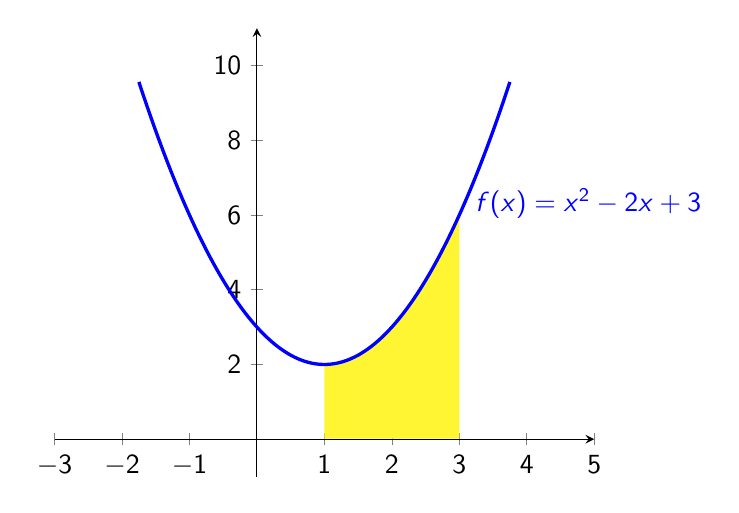
\begin{tikzpicture}
\begin{axis}
[axis lines = middle, xmin = -3, xmax = 5, xtick = {-3,-2,...,5}, ymin = -1, ymax = 11, clip=false]
\addplot [domain = -1.75:3.75, samples=200, blue, very thick, name path = f] {
x^2-2*x+3
} node [right, pos=0.8] {$f(x)=x^2-2x+3$};
\path[name path=axis] (axis cs:-1.5,0.015) -- (axis cs:3,0.015);
\addplot [
        color=yellow!80,
        fill=yellow!80
    ]
    fill between[
        of=f and axis, soft clip={domain=1:3}
    ];
\end{axis}
\end{tikzpicture}
\end{center}
\end{example}

An area that is \emph{below} the $x$-axis has an area that is \textbf{negative}.  \newline\\

The {\color{blue}\textbf{net area}} is the area between the graph of $f(x)$ and the $x$-axis. \newline\\

The {\color{blue}\textbf{gross area}} is the \underline{absolute value} of the region below the $x$-axis.

\begin{example}
For $f(x) = x^3 - x^2 - 4x + 4$,
\begin{enumerate}[(a)]
    \item Sketch and evaluate the net area by computing $\int_{-2}^{2}f(x) \dx$
    \item Calculate the gross area between the graph of $f$ and the $x$-axis.
\end{enumerate}
\end{example}


\end{document}
